\section{Experiments}

For our experiments, we used cluster computers available to us thanks
to Bielefeld University; therefore we cannot make exact claims as to
which CPUs or GPUs we used. \\
Due to time and resource constraints, we were not able to run
experiments over all dimensions. We also decided against training the
models for longer than 10~hours on a single experiment. The time limit
was lifted to 24~hours for experiments in the 3-dimensional case. With
these restrictions, sequence prediction models may not have finished
training or converged (we set a maximum of 1\,000~epochs for all
models; non-sequence predictors trained much faster and never met the
time limit). In the case of 3D~data with only all tile layers
(\texttt{3dtiles}), the sequence prediction models were not able to
train 4~complete epochs in the 24~hour time frame. The transformer in
the same dimensionality was even slower as we had to reduce the batch
size to~1 due to the large memory usage we explained in
section~\ref{sec:generation-via-prediction}\footnote{We could have
  implemented batch sizes of~1 to not be batched but instead remain as
  a singular input (keeping sparsity) to improve performance for this
  special case. However, we decided it was not worth it; we mentioned
  our plans for 3-dimensional sparse arrays fixing most batch-related
  issues all at once in section~\ref{sec:generation-via-prediction}.}.
From the trained models, we take the checkpoint with the lowest test
loss except for the GANs for which we take the checkpoint with the
highest discriminator test loss. The databases we used all consisted
of tile layers only.

We are also not going to take a look at every model in higher
dimensions; internal tests have shown which models work and which
don't. While we \emph{will} contrast LSTMs and transformers, we are
going to only present select models for the other cases. Another
reason is that we do not wish to waste precious public time on the
compute cluster and electricity on models that are very unlikely to
achieve good results. The GANs we use throughout are dense Wasserstein
GAN and the metadata predictors are dense models.

We used the default parameters of each model over all experiments. The
most important parameters are listed in tables~\ref{tab:lstmparams},
\ref{tab:transformerparams}, \ref{tab:ganparams}
and~\ref{tab:metaparams}. For the other values, we point an interested
reader to the source code. \\
The same goes for the training pipelines' parameters, although we will
list these without a table: as mentioned, all pipelines train up to
1\,000 epochs and seed their global random number generator with~0.
The sequence prediction pipeline used a learning rate of~0.0002 and
batch size of~32 with ``hard'' loss and a mean square
error~\cite{MeanSquaredError2019} criterion. The GAN pipeline used a
non-default learning rate of $5 \cdot 10^{-5}$ and the
RMSProp~\cite{tielemannNeuralNetworksMachine2012} optimizer for both
models as well as a batch size of~32 (remember that the Wasserstein
GAN uses no criterion for its loss calculation). The discriminator has
no prior warm-up and trains for one step for each steps of the
generator (so the same amount). The image processing pipeline also
used a non-default learning of $5 \cdot 10^{-5}$, the standard
batch size~32 and a mean square error criterion. \\
For generation, we also set the random seed to~0. In the next
sections, we first look at levels generated by prediction only. After
that, we present the combined pipeline. The levels we will predict on
stay fixed for all experiments; they are levels~257 up to~263 from the
original game. Figure~\ref{fig:predlevels} presents the first two
screens of each of these (for level~261, refer to
figure~\ref{fig:105-detailed} on page~\pageref{fig:105-detailed}). We
make an exception for level~260 and only give its first column as
input. For the complete pipeline generation, for each experiment, we
are going to generate 16~levels and then analyze the first ten levels
with unique numbers that we generate (we never generated fewer than
ten unique numbers).

Earlier tests showed that a larger amount of parameters increased loss
in general and did not lead to decreasing it even after many epochs.
Therefore, with regards to the amount of parameters, we are mostly
confident in our choices. However, due to inexperience with the
transformer models, we may have chosen bad values.

\begin{table}[t]
  \centering
  \makebox[\textwidth]{
    \begin{tabular}[t]{l r r r}
      \toprule
      & \texttt{lstm1d} & \texttt{lstm2d} & \texttt{lstm3dtiles} \\
      \midrule
      \texttt{hiddensize} & \texttt{32} & \texttt{32} & \texttt{64} \\
      \texttt{num\_hiddenlayers} & \texttt{1} & \texttt{2} & \texttt{2} \\
      \texttt{p\_dropout} & \texttt{0.05f0} & \texttt{0.05f0} & \texttt{0.10f0} \\
      \texttt{skipconnections} & \texttt{false} & \texttt{false} & \texttt{false} \\
      \bottomrule
    \end{tabular}
  }%
  \caption{Selected model parameters of the LSTMs; parameter names on
    the y-axis versus model constructors on the x-axis.}
  \label{tab:lstmparams}
\end{table}

\begin{table}[t]
  \centering
  \makebox[\textwidth]{
    \begin{tabular}[t]{l r r r}
      \toprule
      & \texttt{transformer1d} & \texttt{transformer2d} & \texttt{transformer3dtiles} \\
      \midrule
      \texttt{num\_heads} & \texttt{8} & \texttt{8} & \texttt{8} \\
      \texttt{attnhiddensize} & \texttt{4} & \texttt{8} & \texttt{16} \\
      \texttt{ffhiddensize} & \texttt{8} & \texttt{16} & \texttt{32} \\
      \texttt{num\_layers} & \texttt{2} & \texttt{2} & \texttt{3} \\
      \texttt{p\_dropout\_attn} & \texttt{0.05f0} & \texttt{0.05f0} & \texttt{0.10f0} \\
      \texttt{p\_dropout\_ff} & \texttt{0.05f0} & \texttt{0.05f0} & \texttt{0.05f0} \\
      \bottomrule
    \end{tabular}
  }%
  \caption{Selected model parameters of the transformers; parameter
    names on the y-axis versus model constructors on the x-axis.
    ``attn'' is short for attention ``ff'' for feedforward.}
  \label{tab:transformerparams}
\end{table}

\begin{table}[t]
  \centering
  \makebox[\textwidth]{
    \begin{tabular}[t]{l r r r}
      \toprule
      & \texttt{densewsgan1d} & \texttt{densewsgan2d} & \texttt{densewsgan3dtiles} \\
      \midrule
      \texttt{hiddensize} & \texttt{32} & \texttt{64} & \texttt{128} \\
      \texttt{num\_hiddenlayers} & \texttt{3} & \texttt{4} & \texttt{4} \\
      \texttt{clamp\_value} & \texttt{0.01f0} & \texttt{0.01f0} & \texttt{0.01f0} \\
      \texttt{generator\_inputsize} & \texttt{32} & \texttt{96} & \texttt{256} \\
      \texttt{p\_dropout} & \texttt{0.10f0} & \texttt{0.10f0} & \texttt{0.10f0} \\
      \bottomrule
    \end{tabular}
  }%
  \caption{Selected model parameters of the GANs; parameter names on
    the y-axis versus combined constructors on the x-axis (these
    constructors do not actually exist; they are actually separate and
    substitute \texttt{gan} with \texttt{discriminator} or
    \texttt{generator} as appropriate). With the exception mentioned
    below, values apply to both constructors. Clamp values are unique
    to discriminators and generator input sizes are unique to
    generators, therefore these only apply to the appropriate model.}
  \label{tab:ganparams}
\end{table}

\begin{table}[t]
  \centering
  \makebox[\textwidth]{
    \begin{tabular}[t]{l r r r}
      \toprule
      & \texttt{densemeta1d} & \texttt{densemeta2d} & \texttt{densemeta3dtiles} \\
      \midrule
      \texttt{hiddensize} & \texttt{32} & \texttt{32} & \texttt{64} \\
      \texttt{num\_hiddenlayers} & \texttt{1} & \texttt{2} & \texttt{2} \\
      \texttt{p\_dropout} & \texttt{0.05f0} & \texttt{0.10f0} & \texttt{0.10f0} \\
      \bottomrule
    \end{tabular}
  }%
  \caption{Selected model parameters of the metadata predictors;
    parameter names on the y-axis versus model constructors on the
    x-axis (we omitted \texttt{predictor} in the constructor names for
    conciseness).}
  \label{tab:metaparams}
\end{table}

\begin{figure}[t]
  \centering
  \subfloat[Level~257]{%
    \centering
    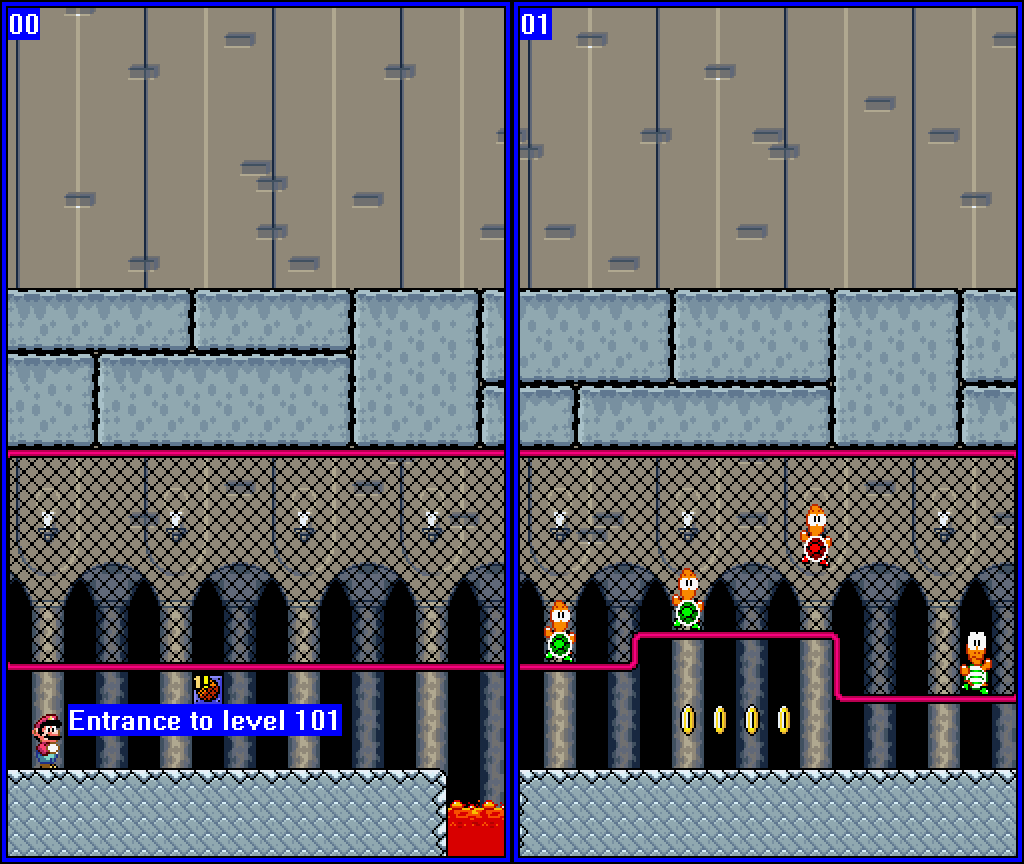
\includegraphics[width=0.5\textwidth]{Level101.png}
  }%
  \subfloat[Level~258]{%
    \centering
    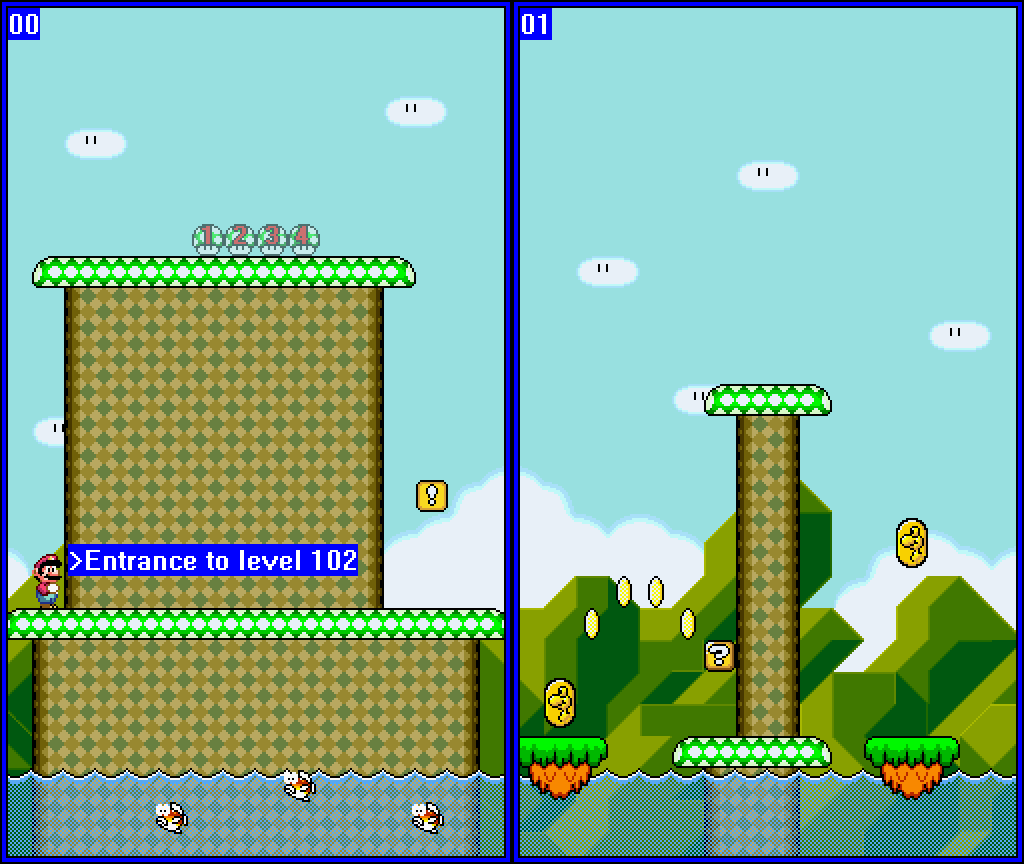
\includegraphics[width=0.5\textwidth]{Level102.png}
  }%
  \\
  \subfloat[Level~259]{%
    \centering
    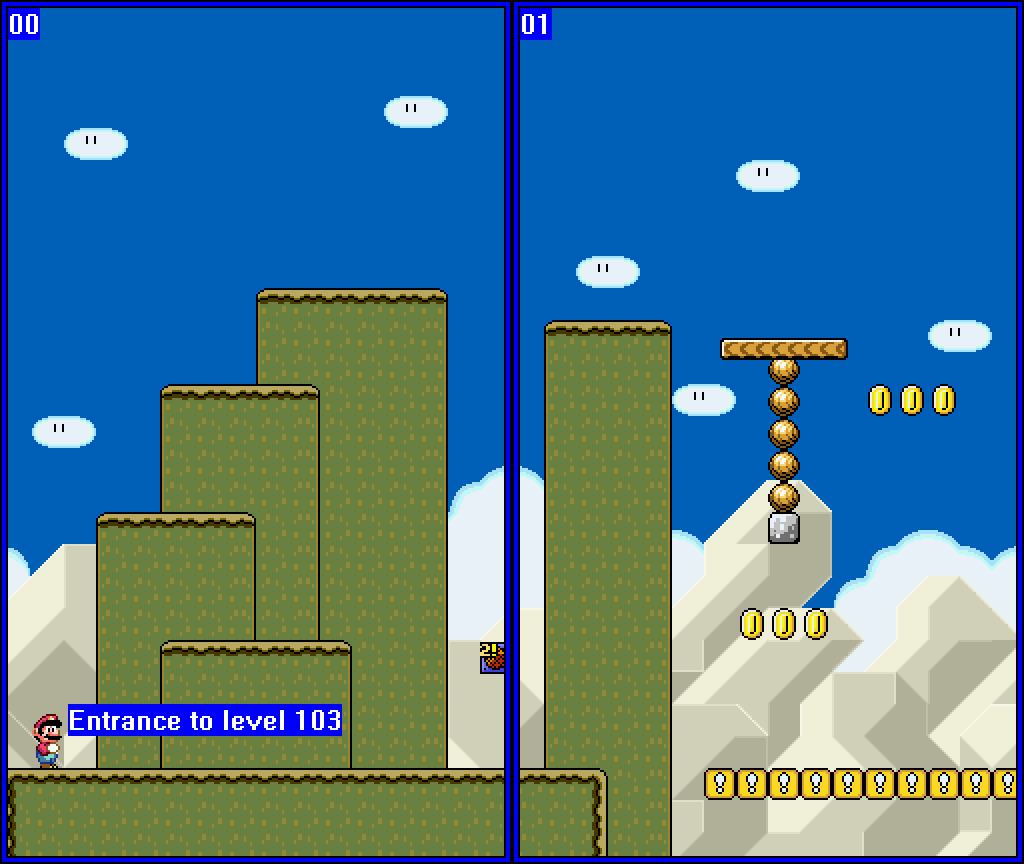
\includegraphics[width=0.5\textwidth]{Level103.png}
  }%
  \subfloat[Level~260]{%
    \centering
    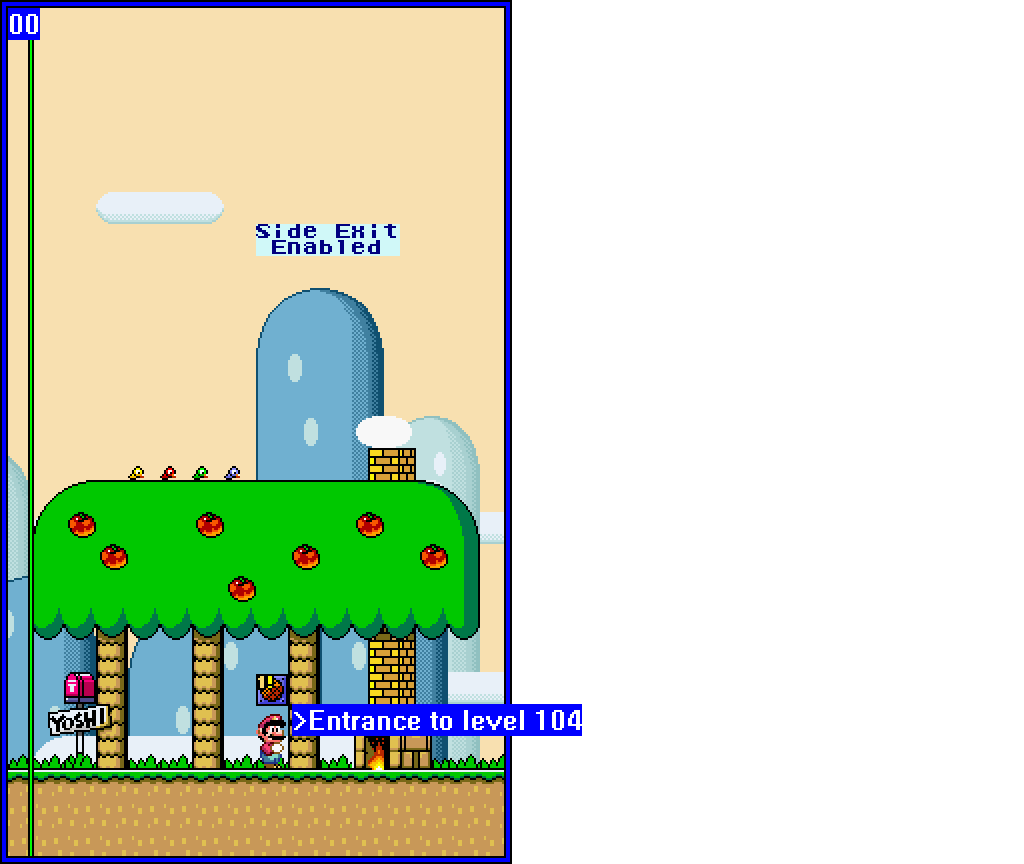
\includegraphics[width=0.5\textwidth]{Level104.png}
  }%
  \\
  \subfloat[Level~262]{%
    \centering
    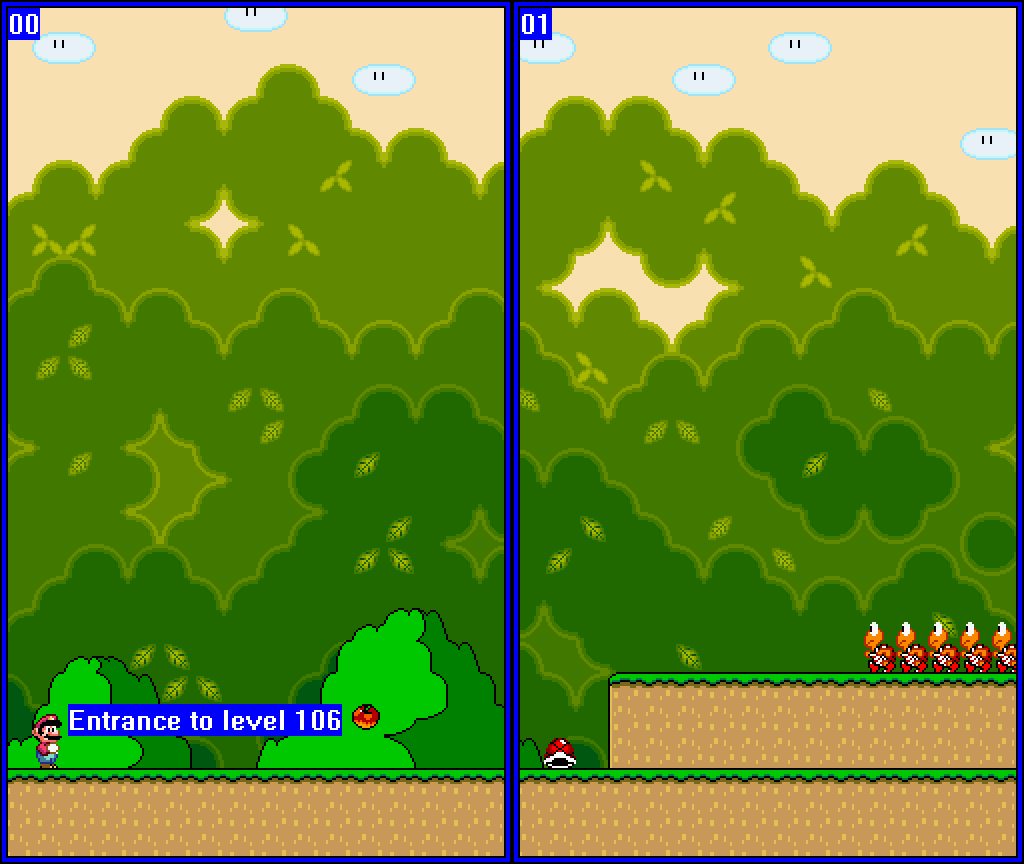
\includegraphics[width=0.5\textwidth]{Level106.png}
  }%
  \subfloat[Level~263]{%
    \centering
    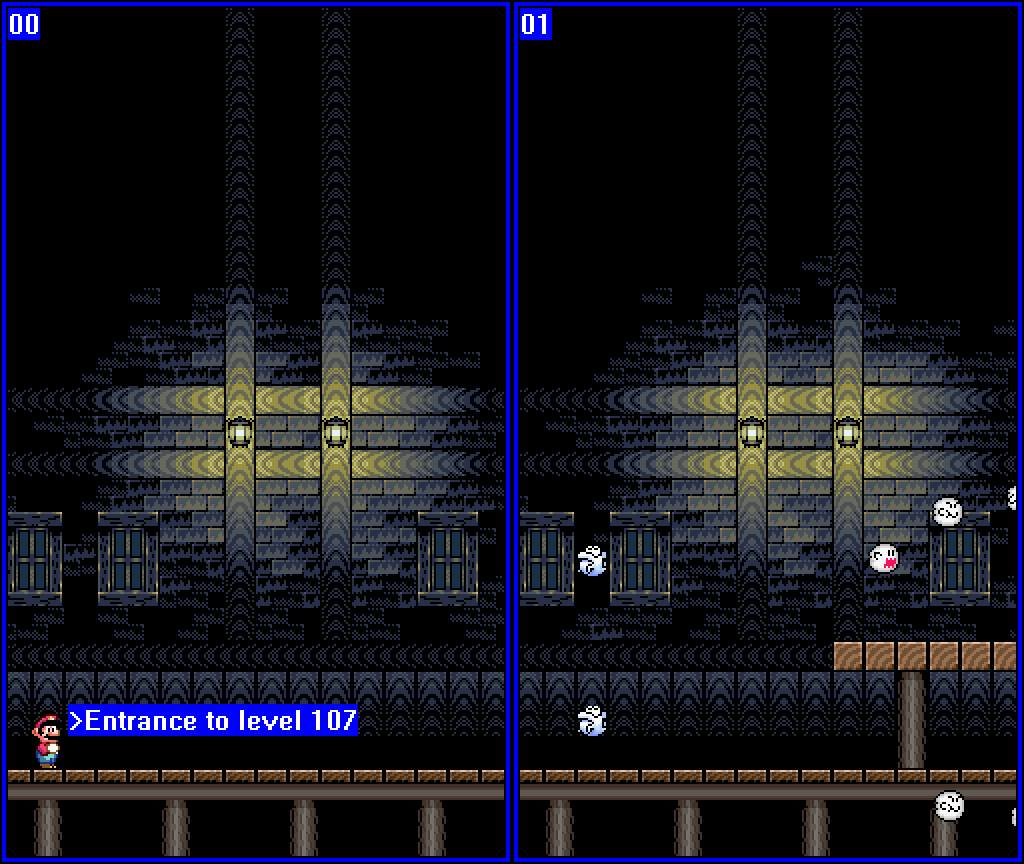
\includegraphics[width=0.5\textwidth]{Level107.png}
  }%
  \caption{The levels we test our sequence prediction models on. For
    level~260, we only use the first column as input, indicated by the
    vertical green line.}
  \label{fig:predlevels}
\end{figure}

\subsection{1-Dimensional}

We trained on a database that did \emph{not} contain squashed data but
where we instead took the row containing the maximum amount of values
over all rows (remember figure~\ref{fig:squash-example} on
page~\pageref{fig:squash-example}).

The LSTM constantly predicts the same tile it saw last (especially
noticeable for level~257 which ends with an empty tile). The exception
is level~260 for which the model predicts empty tiles when the first
screen ends (remember we only gave the first column for this one).

While only changing its generations a bit, the transformer learned to
sometimes first generate empty tiles and then start the same constant
prediction we saw for the LSTM case. The transformer also did not
start predicting emptiness for level~260. What we mentioned above
happened for levels~257 and~258. We show the first two generated
screens of level~258 in figure~\ref{fig:1d-results} (for level~257,
only one column after the first screen was incorrectly predicted to be
zero).
\medskip

\begin{figure}[t]
  \centering
  \subfloat[]{%
    \centering
    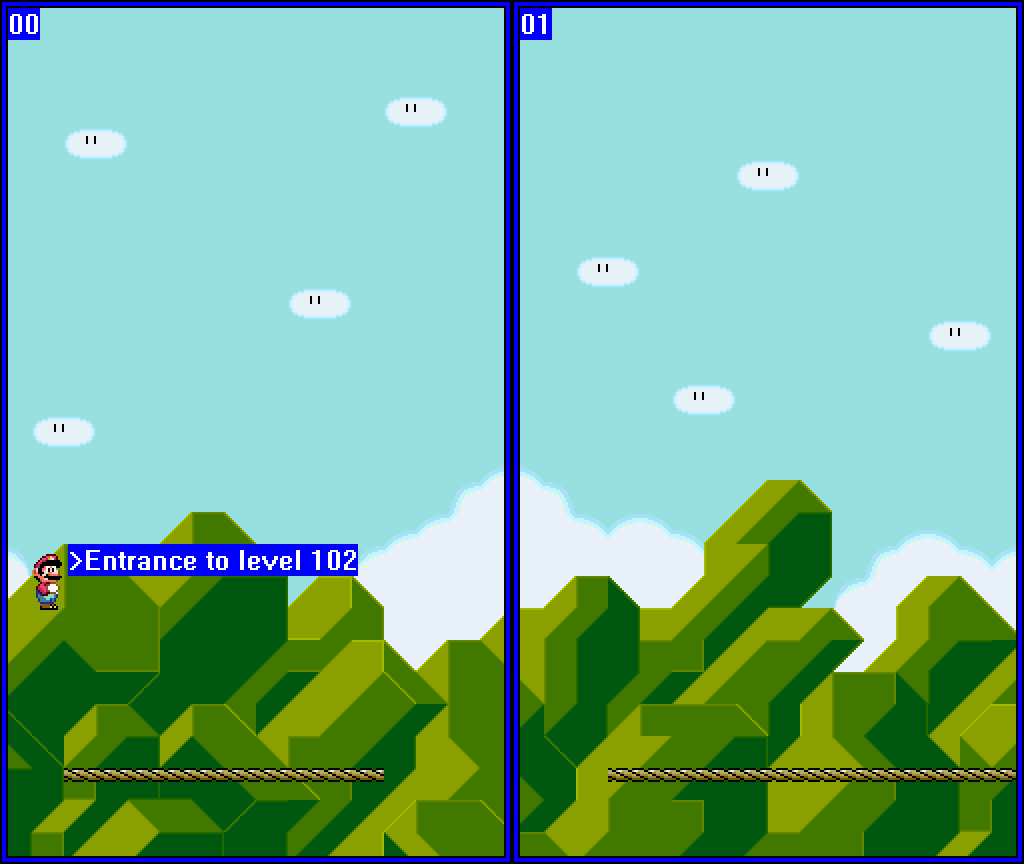
\includegraphics[width=\textwidth]{Level102_gpt_1d_pred.png}
  }%
  \\
  \subfloat[]{%
    \centering
    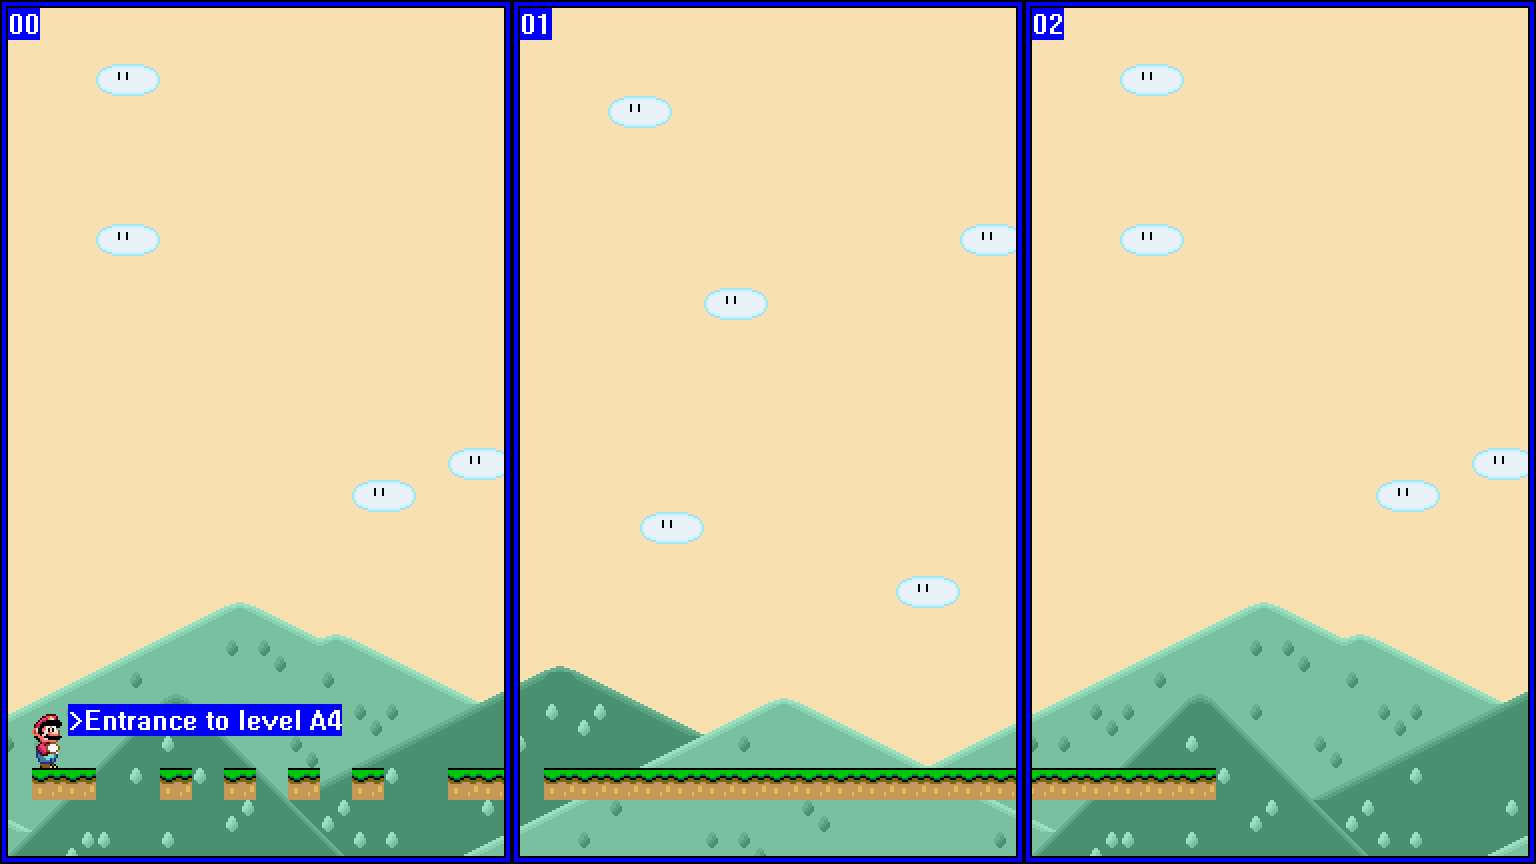
\includegraphics[width=\textwidth]{Level0A4_lstm_1d.png}
  }%
  \caption{Results in the 1-dimensional case. (a)~shows the first two
    screens of level~258 where the second one was predicted by the
    transformer model; (b)~shows a complete level generated by the
    pipeline using the LSTM.}
  \label{fig:1d-results}
\end{figure}

The 1-dimensional pipeline with the LSTM yielded mostly unusable
levels but interesting insights: The GAN created a completely empty
level and others that only contained one ground tile. The metadata
predictor constantly gave the same metadata for these different
generations. Finally, one level was generated that seems to show signs
of progress: in figure~\ref{fig:1d-results} you see a difficult first
screen for which the LSTM did not constantly predict the same column.
Also, everything seen is the whole level~-- the LSTM correctly ended
the level itself. \\
With the transformer, the standalone generations were not as
successful; it constantly predicted ones with no exceptions.

\subsection{2-Dimensional}

In the 2-dimensional case, the LSTM made a solid line of whatever the
last column of the input screen was; just like in the 1-dimensional
predictive case. \\
The transformer started adding (jumpable, although sometimes
difficult) holes after some time for most level. This was sometimes
followed by empty predictions. Only level~102 was a failed generation
as solely empty columns were predicted. We show the predictions for
level~260 in figure~\ref{fig:2d-results}.
\medskip

\begin{figure}[t]
  \centering
  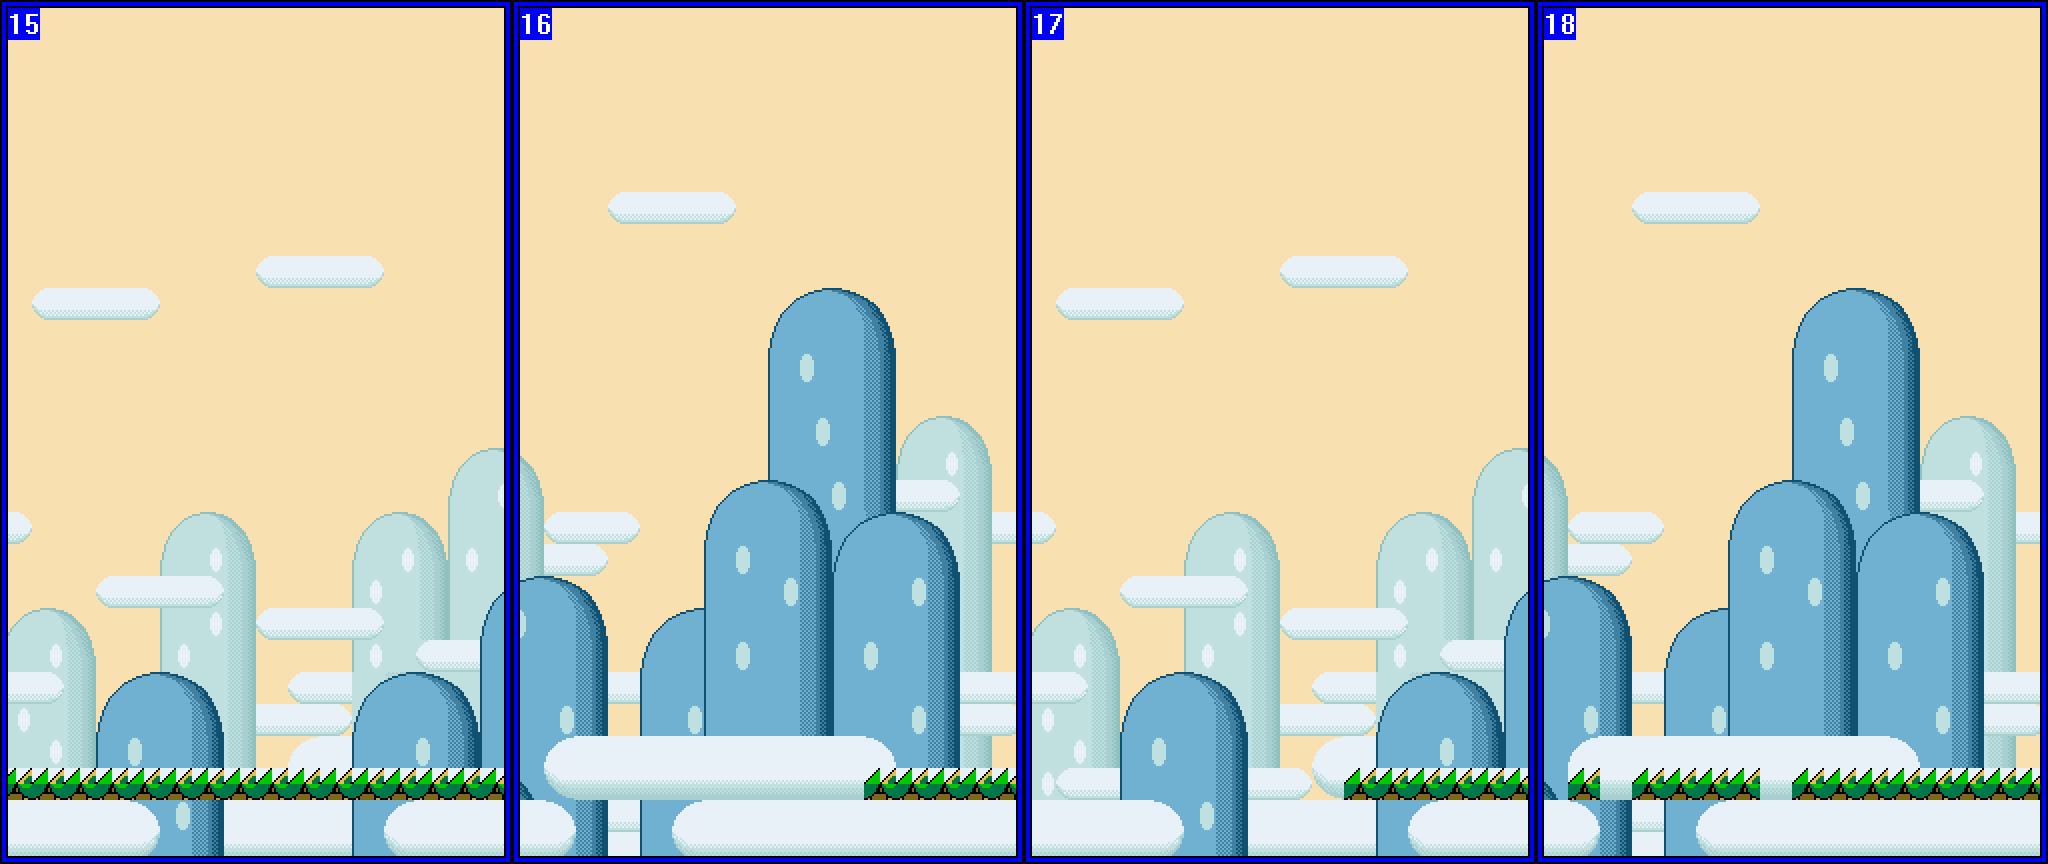
\includegraphics[width=\textwidth]{Level104_gpt_2d_pred.png}
  \caption{Results in the 2-dimensional case: shown are selected
    screens near the end of level~260 as predicted by the transformer
    model. Note that holes were already being generated previously.}
  \label{fig:2d-results}
\end{figure}

Sadly, the generator in the 2-dimensional case only generated empty
first screens; the models then also only predicted emptiness. We then
used another checkpoint, the latest checkpoint of the generator. As
this resulted in segmentation faults with Lunar Magic for the first
level we generated, we then used another checkpoint with high
discriminator test loss. Still, we only got empty first screens with
no predictions. So the only results we have are empty levels.

\subsection{3-Dimensional, Only Tiles}

The 3-dimensional models that trained on layers of tiles only were
already taking very long (too long) to train. In the 24~hours of
training, the latest checkpoint of our LSTM model only had
3\,000~training steps. The transformer model managed 27\,000~steps,
but remember that its batch size was~1 whereas the LSTM trained on
batches of size~32. This means that it actually trained on
significantly less data than the LSTM. For the sake of presenting
results, we will use the LSTM's latest checkpoint. Therefore, note
that these results are not comparable as the transformer was hardly
trained compared to the LSTM.

Mostly due to its low amount of training, the LSTM we trained
generalizes even further than the one from the 2-dimensional case. It
mostly generates tiles one ID above empty tiles (with more training,
this will most likely converge towards empty tiles~-- assuming the
model continues generalizing). These outputs stayed constant except
for level~258 where the model at some points starts to act like the
models presented above and outputs columns of only empty tiles.

The transformer model converges further towards empty tiles than the
LSTM but constantly outputs the same column consisting of a mix of
empty and tiles one ID above empty tiles. Just like with the LSTM,
except for level~258, these outputs stayed constant. However, the mix
clearly shows preference towards the non-empty tiles towards the
bottom of the level suggesting the model learned that these tiles were
more often ``closer'' (in terms of the layers) to tiles with higher
IDs (like ground tiles) than those further above. Even though and
because the transformer only had a fraction of the amount of training
the LSTM enjoyed, we would say that its outputs still had a better
representation of level data.

Interestingly, for both models, the column from which they start
generating empty tiles is at exactly~256 suggesting learning that
levels with a similar first screen are usually only half as long as
others. In the original game, this level has fewer columns.
\medskip

The complete pipeline does not change a lot~-- the GAN generates first
screens that are full of tiles one ID above empty ones. The models
then follow the respective behavior we explained above, although we
have not seen the exceptional behavior of \emph{not} constantly
generating the same column. The metadata predictor has learned to
predict the same tileset for all the levels we analyzed and varied
Mario's entrance position (we saw ``running right'', ``running left'',
``vertical pipe up''). The level numbers predicted were mostly
different but remained below~256. This makes sense given that the
first screens were all very similar (as mentioned in
section~\ref{sec:generating-levels}, the metadata predictor does not
see the same data we see written back as the generated first screen is
not rounded).

%%% Local Variables:
%%% mode: latex
%%% TeX-master: "../SMWLevelGenerator"
%%% End:

